\chapter{Introduction}
\label{chap:Introduction}

\keyterm{ParaView} is an open-source application for visualizing two- and
three-dimensional data sets.  The size of the data sets ParaView can handle
varies widely depending on the architecture on which the application is
run.  The platforms supported by ParaView range from single-processor
workstations to multiple-processor distributed-memory supercomputers or
workstation clusters.  Using a parallel machine, ParaView can process very
large data sets in parallel and later collect the results.  To date, Sandia
National Laboratories has used ParaView to visualize meshes containing up
to 6 billion structured cells and 250 million unstructured cells, and
billions of cells in structured AMR grids.

ParaView’s design contains many conceptual features that make it stand
apart from other scientific visualization solutions.

\begin{itemize}
\item An open-source, scalable, multi-platform visualization application.
\item Support for distributed computation models to process large data sets.
\item An open, flexible, and intuitive user interface.
\item An extensible, modular architecture based on open standards.
\item Commercial maintenance and support.
\end{itemize}

ParaView is used by many academic, government, and commercial institutions
all over the world, and ParaView is downloaded about 3 thousand times each
month.

\begin{inlinefig}
  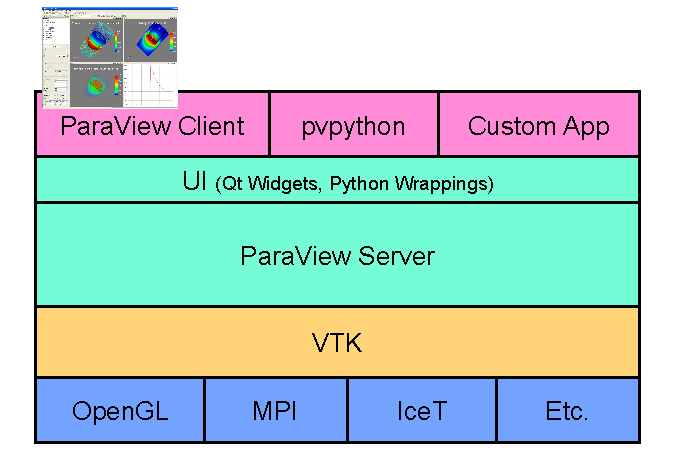
\includegraphics{images/ParaViewLibStack}
\end{inlinefig}

The application most people associate with ParaView is really just a small
client application built on top of a tall stack of libraries that provide
ParaView with its functionality.  Because the vast majority of ParaView
features are implemented in libraries, it is possible to completely replace
the ParaView GUI with your own custom application, as demonstrated in the
following figure.  Furthermore, ParaView comes with a \keyterm{pvpython}
application that allows you to automate the visualization and
post-processing with Python scripting.

Available to each ParaView application is a library of user interface
components to maximize code sharing between them.  A \keyterm{ParaView
  Server} library provides the abstraction layer necessary for running
parallel, interactive visualization.  It relieves the client application
from most of the issues concerning if and how ParaView is running in
parallel.  The \keyterm{Visualization Toolkit} (\keyterm{VTK}) provides the
basic visualization and rendering algorithms.  VTK incorporates several
other libraries to provide basic functionalities such as rendering,
parallel processing, file I/O, and parallel rendering.  Although this
tutorial demonstrates using ParaView through the ParaView client
application, be aware that the modular design of ParaView allows for a
great deal of flexibility and customization.

\section{Development and Funding}

The ParaView project started in 2000 as a collaborative effort between
Kitware Inc. and Los Alamos National Laboratory. The initial funding was
provided by a three year contract with the US Department of Energy ASCI
Views program.  The first public release, ParaView 0.6, was announced in
October 2002.  Development of ParaView continued through collaboration of
Kitware Inc. with Sandia National Laboratories, Los Alamos National
Laboratories, the Army Research Laboratory, and various other academic and
government institutions.

In September 2005, Kitware, Sandia National Labs and CSimSoft started the
development of ParaView 3.0. This was a major effort focused on rewriting
the user interface to be more user friendly and on developing a
quantitative analysis framework. ParaView 3.0 was released in May 2007.

Development of ParaView continues today.  Sandia National Laboratories
continues to fund ParaView development through the ASC project.  ParaView
is integrated as the major development platform for SciDAC Institute for
Ultra-Scale Visualization
(\href{http://www.ultravis.org}{www.ultravis.org}).  The US Department of
Energy also funds ParaView through Los Alamos National Laboratories, an
Army SBIR, and an ERDC contract.  The US National Science Foundation also
funds ParaView with an SBIR.  Other institutions also have ParaView support
contracts: Electricity de France, Mirarco, and oil industry customers.
Also, because ParaView is an open source project, other institutions such
as the Swiss National Supercomputing Centre contribute back their own
development.

\section{Basics of Visualization}

\begin{inlinefig}
  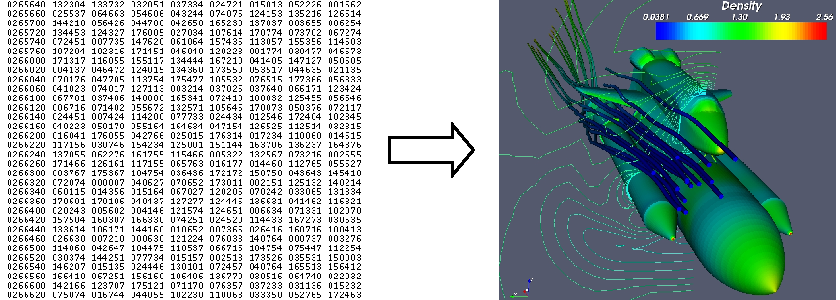
\includegraphics[width=\linewidth]{images/BasicsOfVisualization}
\end{inlinefig}

Put simply, the process of visualization is taking raw data and converting
it to a form that is viewable and understandable to humans.  This allows us
to get a better cognitive understanding of our data.  Scientific
visualization is specifically concerned with the type of data that has a
well defined representation in 2D or 3D space.  Data that comes from
simulation meshes and scanner data is well suited for this type of
analysis.

There are three basic steps to visualizing your data: reading, filtering,
and rendering.  First, your data must be read into ParaView.  Next, you may
apply any number of \keyterm{filters} that process the data to generate,
extract, or derive features from the data.  Finally, a viewable image is
rendered from the data.

ParaView was designed primarily to handle data with spatial
representation. Thus the primary \keyterm{data types} used in ParaView are
meshes.

\noindent
\begin{tabularx}{\linewidth}{p{2in}X}
  \parbox{2in}{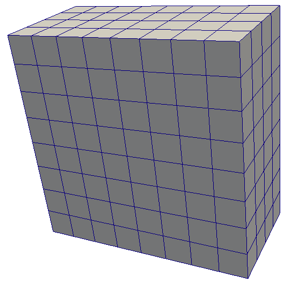
\includegraphics[width=2in]{images/ImageData}} &
  \begin{minipage}{\linewidth}
    \keyterm{Uniform Rectilinear (Image Data)}

    A uniform rectilinear grid is a one- two- or three- dimensional array of
    data.  The points are orthonormal to each other and are spaced regularly
    along each direction.
  \end{minipage}
\end{tabularx}

\noindent
\begin{tabularx}{\linewidth}{p{2in}X}
  \parbox{2in}{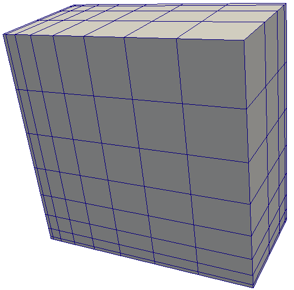
\includegraphics[width=2in]{images/RectilinearGrid}} &
  \begin{minipage}{\linewidth}
    \keyterm{Non-uniform Rectilinear (Rectilinear Grid)}

    Similar to the uniform rectilinear grid except that the spacing between
    points may vary along each axis.
  \end{minipage}
\end{tabularx}

\noindent
\begin{tabularx}{\linewidth}{p{2in}X}
  \parbox{2in}{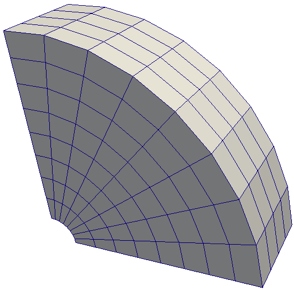
\includegraphics[width=2in]{images/StructuredGrid}} &
  \begin{minipage}{\linewidth}
    \keyterm{Curvilinear (Structured Grid)}

    Curvilinear grids have the same topology as rectilinear grids.
    However, each point in a curvilinear grid can be placed at an arbitrary
    coordinate (provided that it does not result in cells that overlap or
    self intersect).  Curvilinear grids provide the more compact memory
    footprint and implicit topology of the rectilinear grids, but also
    allow for much more variation in the shape of the mesh.
  \end{minipage}
\end{tabularx}

\noindent
\begin{tabularx}{\linewidth}{p{2in}X}
  \parbox{2in}{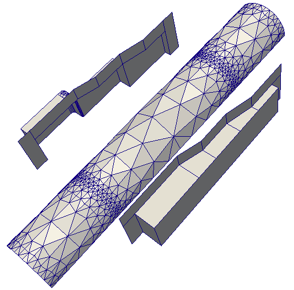
\includegraphics[width=2in]{images/PolyData}} &
  \begin{minipage}{\linewidth}
    \keyterm{Polygonal (Poly Data)}

    Polygonal data sets are composed of points, lines, and 2D polygons.
    Connections between cells can be arbitrary or non-existent.
    
    Polygonal data represents the basic rendering primitives.  Any data
    must be converted to polygonal data before being rendered (unless
    volume rendering is employed), although ParaView will automatically
    make this conversion.
  \end{minipage}
\end{tabularx}

\noindent
\begin{tabularx}{\linewidth}{p{2in}X}
  \parbox{2in}{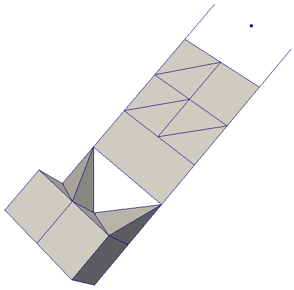
\includegraphics[width=2in]{images/UnstructuredGrid}} &
  \begin{minipage}{\linewidth}
    \keyterm{Unstructured Grid}

    Unstructured data sets are composed of points, lines, 2D polygons, 3D
    tetrahedra, and nonlinear cells.  They are similar to polygonal data
    except that they can also represent 3D tetrahedra and nonlinear cells,
    which cannot be directly rendered.
  \end{minipage}
\end{tabularx}

In addition to these basic data types, ParaView also supports
\keyterm{multi-block} data.  A basic multi-block data set is created
whenever data sets are grouped together or whenever a file containing
multiple blocks is read.  ParaView also has some special data types for
representing \keyterm{Hierarchical Adaptive Mesh Refinement}
(\keyterm{AMR}), \keyterm{Hierarchical Uniform AMR}, \keyterm{Octree},
\keyterm{Tablular} and \keyterm{Graph} type data sets


\section{More Information}

There are many places to find more information about ParaView.  For
starters, ParaView has online help that can be accessed by simply clicking
the \icon{pqHelp32} button in the application.  In addition to the on-line
help, \emph{The ParaView Guide} written by Amy Henderson Squillacote and
available from Kitware is a helpful guide for all things ParaView.

The ParaView web page, \href{http://www.paraview.org}{www.paraview.org}, is
also an excellent place to find more information about ParaView.  From
there you can find helpful links to mailing lists, Wiki pages, and
frequently asked questions as well as information about professional
support services.



% Chapter Introduction
